\section{Semantic Translation of Blocks}
\label{sec:trans}

In this section, we focus on the methodology to map individual Simulink blocks to designs in UTP semantically. Basically, a block or subsystem is regarded as a relation between inputs and outputs. We use an undashed variable and a dashed variable to denotes input signals and output signals respectively.

\subsection{State Space}
The state space of our theory for block diagrams is composed of only one variable in addition to $ok$, named $inouts$. Originally, we defined it as a function from real numbers (time $t$) to a list of inputs or outputs. Each element in the list denotes an input or output and their order in the list is the order of input or output signals.
\begin{align*}
    inouts: \real_{\geq 0}\fun \seq \real
\end{align*}

However, according to our single-rate assumption, the timestamp at time $t$ is equal to multiples of a basic period $T$: $inouts(t) = inouts(n*T)$. Then $T$ is abstracted away and only the step number $n$ is related. Finally, it is defined below.

\begin{align*}
    inouts : \nat \fun \seq \real
\end{align*}

Then a block is a design that establishes the relation between an initial observation $inouts$ (a list of input signals) and a final observation $inouts'$ (a list of output signals). Additionally, this is subject to the assumption of the design.

\subsection{Healthiness Condition: $\healthy{SimBlock}$}
This healthiness condition characterises a block with a fixed number of inputs and outputs. Additionally it is feasible. A design is a feasible block if there exists at least a pair of $inouts$ and $inouts'$ that establishes both the precondition and postcondition of the design.

\begin{definition}[$\healthy{SimBlock}$]
    A design $P$ with $m$ inputs and $n$ outputs is a Simulink block if $P$ is $\healthy{SimBlock}$ healthy.
    \begin{align*}
       \healthy{SimBlock}(m, n, P) \defs \left( 
       \begin{array}[]{l}
       \left(pre_D(P) \land post_D(P) \neq \false\right) \land \\
       \left(\left(\forall n @ \#\left(inouts~n\right) = m\right) \refinedby Dom~\left(pre_D(P) \land post_D(P)\right)\right) \\
       \left(\left(\forall n @ \#\left(inouts~n\right) = n\right) \refinedby Ran~\left(pre_D(P) \land post_D(P)\right)\right)
       \end{array}\right)
    \end{align*}
    where $Dom$ and $Ran$ calculate the characteristic predicate for domain and range. Their definitions are shown below.
    \begin{align*}
       &Dom(P) \defs \left(\exists inouts' @ P\right) & \\  
       &Ran(P) \defs \left(\exists inouts @ P\right) &
    \end{align*}
\end{definition}

$inps$ and $outps$ are the operators to get the number of input signals and output signals for a block. They are implied from $\healthy{SimBlock}$ of the block. 
\begin{definition}[$inps$ and $outps$]
\begin{align*}
   \healthy{SimBlock}(m, n, P) \implies \left(inps(P) = m \land outps(P) = n\right) 
\end{align*}
    Provided that $P$ is a healthy block, $inps$ returns the number of its inputs and $outps$ returns the number of its outputs.
\end{definition}

\subsection{Blocks}
In order to give definitions of the corresponding designs for Simulink blocks, firstly we define a design pattern $FBlock$. Then we illustrate definitions of two typical Simulink blocks and three additional virtual blocks using this pattern. The definitions of all other blocks could be found in Appendix~\ref{sec:block_theories}.

\subsubsection{Pattern}
We defined a pattern that is used to define all other blocks.
\begin{definition}[$FBlock$]
\begin{align*}
    & FBlock\left(f_1, m, n, f_2\right) &\\
    &\defs \left(
            \vdesign{\forall nn @ f_1\left(inouts, nn\right)}
                    {\forall nn @ \left(
                        \begin{array}[]{l}
                            \#\left(inouts(nn)\right) = m \land \\
                            \#\left(inouts'(nn)\right) = n \land \\
                            \left(inouts'(nn) = f_2\left(inouts'(nn), nn\right)\right) \land \\ 
                            \left(\forall sigs:\nat \fun \seq~\real, nn:\nat @ \#\left(sigs~nn\right) = m \implies \#\left(f_2(sigs, nn)\right) = n\right)
                        \end{array} \right)
                    }
        \right) &
\end{align*}
\end{definition}

$FBlock$ has four parameters: $f_1$ is a predicate that specifies the assumption of the block and it is a function on input signals; $m$ and $n$ are the number of inputs and outputs, and $f_2$ is a function that relates inputs to outputs and is used to establish the postcondition of the block. The precondition of $FBlock$ states that $f_1$ holds for inputs at any step $nn$. And the postcondition specifies that for any step $nn$ the block always has $m$ inputs and $n$ outputs, the relation between outputs and inputs are given by $f_2$, and additionally $f_2$ always produces $n$ outputs provided there are $m$ inputs.

\subsubsection{Simulink Blocks}
\begin{definition}[Unit Delay] \label{def:ud}
    \begin{align*}
        UnitDelay\left(x_0\right) \defs FBlock\left( \logtrue{f}, 1, 1, \left(\lambda x, n @ \langle \condition{x_0}{n = 0}{hd\left(x~(n-1)\right)}\rangle\right)\right) 
    \end{align*}
    where $hd$ is an operator to get the head of a sequence, and $\logtrue{f} = \left(\lambda x, n @ \logtrue{}\right)$ that means no constraints on input signals.
\end{definition}
The definition \ref{def:ud} of the Unit Delay block is straightforward: it accepts all inputs, has one input and one output, and produces initial value $x_0$ in its first step (0) and the previous input otherwise.

\begin{definition}[Product (Divide)] \label{def:div2}
    \begin{align*}
        Div2 \defs FBlock\left( \left(\lambda x, n @ hd(tl(x~n)) \neq 0\right), 2, 1, \left(\lambda x, n @ \langle hd(x~n)/hd(tl(x~n))\rangle\right)\right) 
    \end{align*}
    where $tl$ is an operator to get the tail of a sequence.
\end{definition}
The definition \ref{def:div2} of Divide block is slightly different because it assumes the input value of its second input signal is not zero at any step. By this way, the precondition enables modelling of non-input-receptive systems that may reject some inputs at some points. %That is the similar case for the square root function in the math block.

\subsubsection{Virtual Blocks}
In addition to Simulink blocks, we have introduced three blocks for the purpose of composition: $Id$, $Split2$, and $Router$. The usage of these blocks is illustrated in Figure~\ref{fig:compose}.

\begin{definition}[Id] \label{def:id}
    \begin{align*}
        Id \defs FBlock\left( \logtrue{f}, 1, 1, \left(\lambda x, n @ \langle hd\left(x~n\right)\rangle\right)\right) 
    \end{align*}
\end{definition}
The identity block $Id$ is a block that has one input and one output, and the output value is always equal to the input value. It establishes a fact that a direct signal line in Simulink could be treated as sequential composition of many $Id$ blocks. The usage of $Id$ is shown in Figure~\ref{fig:id}.

\begin{definition}[Split2]  \label{def:split2}
    \begin{align*}
        Split2 \defs FBlock\left( \logtrue{f}, 1, 2, \left(\lambda x, n @ \langle hd\left(x~n\right), hd\left(x~n\right)\rangle\right)\right) 
    \end{align*}
\end{definition}
$Split2$ corresponds to the signal connection splitter that produces two signals from one and both signals are equal to the input signal. The usage of $Split2$ is shown in Figure~\ref{fig:split}.

\begin{definition}[Router] \label{def:router} 
    \begin{align*}
        Router\left(m, table\right) \defs FBlock\left( \logtrue{f}, m, m, \left(\lambda x, n @ reorder\left(\left(x~n\right), table\right)\right)\right) 
    \end{align*}
\end{definition}
$Router$ corresponds to the crossing connection of signals and this virtual block changes the order of input and output signals according to the supplied table. The usage of $Router$ is shown in Figure~\ref{fig:router}.

\subsection{Subsystems}
The treatment of subsystems (no matter whether hierarchical subsystems or atomic subsystems) in our designs is similar to that of blocks. They could be regarded as a bigger black box that relates inputs to outputs.

\section{Block Compositions}
\label{sec:comp}

In this section, we define three composition operators that are used to compose subsystems or systems from blocks. We also use three virtual blocks to map Simulink's connections in our designs.

For all definitions and laws in this section, if there are no special notes, we assume the following predicates. 
\begin{align*}
    & \healthy{SimBlock}\left(m_1, n_1, P_1\right) & \\
    & \healthy{SimBlock}\left(m_2, n_2, P_2\right) & \\
    & \healthy{SimBlock}\left(m_3, n_3, P_3\right) & \\
    & \healthy{SimBlock}\left(m_1, n_1, Q_1\right) & \\
    & \healthy{SimBlock}\left(m_2, n_2, Q_2\right) & \\
    & P_1 \refinedby Q_1 & \\
    &P_2 \refinedby Q_2 &
\end{align*}

\begin{figure}[htb!]
    \captionsetup[subfigure]{justification=centering}
    \centering 
    \begin{subfigure}[t]{0.3\textwidth}
        \centering 
        \begin{tikzpicture}[auto, node distance=2cm,>=latex']
            \node [input, name=input1] (input1) {};
            \node [block, right of=input1, node distance=1.5cm] (b1) {B1};
            \node [block, below of=b1, dashed] (id) {Id};
            \node [input, left of=id, node distance=1.5cm] (input2) {};
            \node [block, minimum height=8em] (b2) at ([xshift=2cm, yshift=-1cm]b1){B2};
            \draw [->] (input1) -- (b1);
            \draw [->] (b1) -- (b1 -| b2.west);
            \draw [->] (input2) -- (input2 -| b2.west);
        \end{tikzpicture}
        \caption{Id}
        \label{fig:id}
    \end{subfigure}
    \begin{subfigure}[t]{0.3\textwidth}
        \centering 
        \begin{tikzpicture}[auto, node distance=2cm,>=latex']
            \node [input, name=input1] (input1) {};
            \node [block, right of=input1, node distance=2.5cm] (b1) {B1};
            \node [block, below of=b1] (b2) {B2};
            \draw [->] (input1) --node[name=z,anchor=north]{} (b1);
            \node [block, dashed] (split) at (z) {Split};
            \draw [->] (input1) -- (b1);
            \draw [->] (z) |- (b2);
        \end{tikzpicture}
        \caption{Split}
        \label{fig:split}
    \end{subfigure}
    \begin{subfigure}[t]{0.3\textwidth}
        \centering 
        \begin{tikzpicture}[auto, node distance=2cm,>=latex']
            \begin{pgfonlayer}{fg}
                \node [input, name=input1] (input1) {};
                \node [block, right of=input1, node distance=3cm] (b1) {B1};
                \node [block, below of=b1] (b2) {B2};
                \node [input, left of=b2, node distance=3cm] (input2) {};
                \node [block, dashed, minimum height=8em] (router) at ([xshift=1.5cm, yshift=-1cm]input1.east) {Router};
                %\node [output, right of=b1, node distance=1.5cm] (output1) {};
                %\node [output, right of=b2, node distance=1.5cm] (output2) {};
                \draw [->] (input1) --node[name=z1]{} (b1);
                \draw [->] ([xshift=0.5cm]input1) -- (b2);
                %\draw [->] (z1) -- (b2);
                \draw [->] (input2) --node[name=z2]{} (b2);
                \draw [->] ([xshift=0.5cm]input2) -- (b1);
                %\draw [->] (z2) -- (b1);
                %\draw [->] (z1 |- b2.west) -- (z1 -| b2.west);
                %\draw [->] (z2 |- b1.west) -- (z2 -| b1.west);
                %\draw [->] (b2) -- (output2);
            \end{pgfonlayer}
            \begin{pgfonlayer}{bg}
                \node [rectangle, dashed, fit= (b1) (b2), label=left:] {};
            \end{pgfonlayer}
        \end{tikzpicture}
        \caption{Router}
        \label{fig:router}
    \end{subfigure}
    \begin{subfigure}[t]{0.3\textwidth}
        \centering 
        \begin{tikzpicture}[auto, node distance=2cm,>=latex']
            \begin{pgfonlayer}{fg}
                \node [input, name=input1] (input1) {};
                \node [block, right of=input1, node distance=1.5cm] (b1) {B1};
                \node [block, right of=b1] (b2) {B2};
                \node [output, right of=b2, node distance=1.5cm] (output) {};
                \draw [->] (input1) -- (b1);
                \draw [->] (b1) -- (b2);
                \draw [->] (b2) -- (output);
            \end{pgfonlayer}
            \begin{pgfonlayer}{bg}
                \node [rectangle, draw, dashed, fit= (b1) (b2), label=left:] {};
            \end{pgfonlayer}
        \end{tikzpicture}
        \caption{Sequential Composition}
        \label{fig:seq_comp}
    \end{subfigure}
    \begin{subfigure}[t]{0.3\textwidth}
        \centering 
        \begin{tikzpicture}[auto, node distance=2cm,>=latex']
            \begin{pgfonlayer}{fg}
                \node [input, name=input1] (input1) {};
                \node [block, right of=input1, node distance=1.5cm] (b1) {B1};
                \node [block, below of=b1] (b2) {B2};
                \node [input, left of=b2, node distance=1.5cm] (input2) {};
                \node [output, right of=b1, node distance=1.5cm] (output1) {};
                \node [output, right of=b2, node distance=1.5cm] (output2) {};
                \draw [->] (input1) -- (b1);
                \draw [->] (b1) -- (output1);
                \draw [->] (input2) -- (b2);
                \draw [->] (b2) -- (output2);
            \end{pgfonlayer}
            \begin{pgfonlayer}{bg}
                \node [rectangle, draw, dashed, fit= (b1) (b2), label=left:] {};
            \end{pgfonlayer}
        \end{tikzpicture}
        \caption{Parallel Composition}
        \label{fig:par_comp}
    \end{subfigure}
    \begin{subfigure}[t]{0.3\textwidth}
        \centering 
        \begin{tikzpicture}[auto, node distance=2cm,>=latex']
            \node [input, name=input1] (input1) {};
            \node [input, below of=input1] (input2) {};
            \node [block, minimum height=6em] (b1) at ([xshift=2cm, yshift=-1cm]input1){B};
            \node [tmp, above of=b1] (tmp1){};
            \node [output, right of=input1, node distance=4cm] (output1) {};
            \node [output, right of=input2, node distance=4cm] (output2) {};
            %\draw [->] (input1) -- (input1 -| b1.west);
            %\draw [->] (input2) -- (input2 -| b1.west);
            %\draw [->] (b1.east) |- (output1) |- (temp1) -| (input1) -- (input1 -| b1.west);
            \draw [->] ([yshift=0.5cm]b1.east) -- ++(0.7cm, 0) -- ++(0,1.1cm) -- ++(-2.6cm, 0) -- ++(0,-1.1cm) -- ([yshift=0.5cm]b1.west);
            \draw [->] ([yshift=-0.5cm]b1.east) -- ++(1cm,0); 
            \draw [->] ([xshift=-1cm, yshift=-0.5cm]b1.west) -- ([yshift=-0.5cm]b1.west); 
        \end{tikzpicture}
        \caption{Feedback}
        \label{fig:fd_comp}
    \end{subfigure}
    \caption{Composition of Blocks}\label{fig:compose}
\end{figure}


\subsection{Sequential Composition}
The meaning of sequential composition of designs is defined in Theorem~\ref{thm:des_seq}. It corresponds to composition of two blocks in Figure~\ref{fig:seq_comp} where the outputs of $B_1$ are equal to the inputs of $B_2$.

Provided 
   \begin{align*}
       \begin{array}[]{ll}
           P = \left(FBlock\left( \logtrue{f}, m_1, n_1, f_1\right)\right) & \qquad \healthy{SimBlock}\left(m_1, n_1, P\right) \\ 
           Q = \left(FBlock\left( \logtrue{f}, n_1, n_2, f_2\right)\right) & \qquad \healthy{SimBlock}\left(n_1, n_2, Q\right) \\ 
       \end{array}
   \end{align*}

The expansion law of sequential composition is given below.
\begin{theorem}[Expansion]
   \begin{align*}
       &\left(P \dcomp Q \right) = FBlock\left( \logtrue{f}, m_1, n_2, (f_2 \circ f_1)\right) & \tag*{[Expansion]}
   \end{align*}
    \label{thm:seq_exp}
\end{theorem}
This theorem establishs that sequential composition of two blocks, where the number of outputs of the first block is equal to the number of inputs of the second block, is simply a new block with the same number of inputs as the first block $P$ and the same number of outputs as the second block $Q$, and additionally the postcondition of this composed block is function composition. In addition, the composed block is still $\healthy{SimBlock}$ healthy which is shown in the closure theorem below.

\begin{theorem}[Closure]
   \begin{align*}
       &\healthy{SimBlock}\left(m_1, n_2, \left(P \dcomp Q \right)\right) & \tag*{[\healthy{SimBlock} Closure]} 
   \end{align*}
    \label{thm:seq_closure}
\end{theorem}

\subsection{Parallel Composition}
Parallel composition of two blocks is a stack of inputs and outputs from both blocks and is illustrated in Figure~\ref{fig:par_comp}. It is defined below.
\begin{definition}[Parallel Composition] \label{def:parallelB} 
    \begin{align*}
        P \parallel_{B} Q \defs \left(
        \begin{array}[]{l}
            \left(takem (inps(P)+inps(Q))~inps(P) \dcomp P \right) \\
            \parallel_{B_M} \\
            \left(dropm (inps(P)+inps(Q))~inps(P) \dcomp Q \right) 
        \end{array} \right)
    \end{align*}
\end{definition}
where $takem$ and $dropm$ are two blocks to split inputs into two parts and their definitions can be found in Appendix~\ref{sec:block_theories}, and $B_M$ is defined below. 
\begin{definition}[$B_M$] \label{def:mergeB} 
    \begin{align*}
        B_M \defs \left(ok' = 0.ok \land 1.ok\right) \land \left(inouts' = 0.inouts \cat 1.inouts\right) 
    \end{align*}
\end{definition}

The definition of parallel composition~\ref{def:parallelB} for designs is similar to the parallel-by-merge scheme~\cite[Sect.~7.2]{Hoare1998} in UTP. Parallel-by-merge is denoted as $P \parallel_M Q$ where $M$ is a special relation that explains how the output of parallel composition of $P$ and $Q$ should be merged following execution. 

However, parallel-by-merge assumes that the initial observations for both predicates should be the same. But that is not the case for our block composition because the inputs to the first block and that to the second block are different. Therefore, in order to use the parallel by merge, firstly we need to partition the inputs to the composition into two parts: one to the first block and another to the second block. This is illustrated in Figure~\ref{fig:parallel} where we assume that $P$ has $m$ inputs and $i$ outputs, and $Q$ has $n$ inputs and $j$ outputs. Finally, it has the same inputs ($m+n$) and the outputs of $P$ and $Q$ are merged by $B_M$ to get $i+j$ outputs.

\begin{figure}[htb]
    \begin{center}
        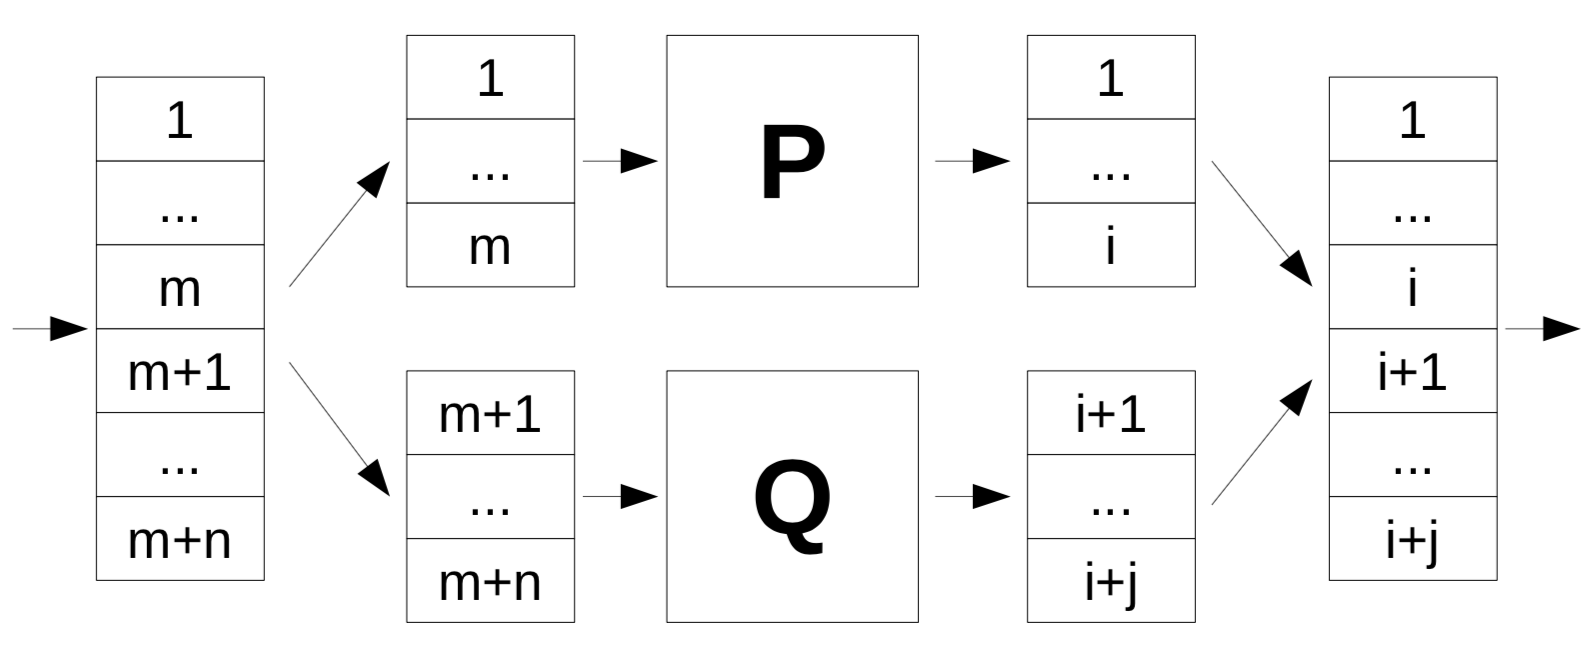
\includegraphics[scale=0.45]{parallel}
    \end{center}
    \caption{Parallel Composition of Two Blocks}
    \label{fig:parallel}
\end{figure}

The merge operator $B_M$ states that the parallel composition terminates if both blocks terminate. And on termination, the output of parallel composition is concatenation of the outputs from the first block and the outputs from the second block. $takem$ and $dropm$ are two blocks that have the same inputs and the number of inputs is equal to addition of the number inputs of $P$ and the number inputs of $Q$. $takem$ only takes the first part of inputs as required by $P$, and $dropm$ takes the second part of inputs as required by $Q$.

\begin{theorem}[Associativity, Monotonicity, and $\healthy{SimBlock}$ Closure]
    \begin{align*}
        & P_1 \parallel_B \left(P_2 \parallel_B P_3\right) = \left(P_1 \parallel_B P_2\right) \parallel_B P_3 & \tag*{[Associativity]} \\
        & \left(P_1 \parallel_B Q_1\right) \refinedby \left(P_2 \parallel_B Q_2\right) & \tag*{[Monotonicity]} \\ 
        & \healthy{SimBlock}\left(m1+m2, n1+n2, \left(P_1 \parallel_B P_2\right)\right) & \tag*{[\healthy{SimBlock} Closure]} \\ 
        & inps\left(P_1 \parallel_B P_2\right) = m_1 + m_2 & \tag*{} \\
        & outps\left(P_1 \parallel_B P_2\right) = n_1 + n_2 & \tag*{}
    \end{align*}
    \label{thm:parallelB}
\end{theorem}

Parallel composition is associative, monotonic in terms of the refinement relation, and $\healthy{SimBlock}$ healthy. The inputs and outputs of parallel composition are combination of the inputs and outputs of both blocks.

\begin{theorem}[Parallel Operator Expansion]
   Provided 
   \begin{align*}
       \begin{array}[]{ll}
           P = \left(FBlock\left( \logtrue{f}, m_1, n_1, f_1\right)\right) & \qquad \healthy{SimBlock}\left(m_1, n_1, P\right) \\ 
           Q = \left(FBlock\left( \logtrue{f}, m_2, n_2, f_2\right)\right) & \qquad \healthy{SimBlock}\left(m_2, n_2, Q\right) \\ 
       \end{array}
   \end{align*}
   then, 
   \begin{align*}
       \left(P \parallel_B Q\right) = & FBlock\left(
       \begin{array}[]{l}
            \logtrue{f}, m_1+m_2, n_1+n_2, \\
            \left(\lambda x, n @ 
                \left(
                \begin{array}[]{l}
                    \left(f_1 \circ \left(\lambda x, n @ take\left(m_1, x~n\right)\right)\right) \\
                    \cat \left(f_2 \circ \left(\lambda x, n @ drop\left(m_1, x~n\right)\right)\right) 
                \end{array}\right)\right) \\
       \end{array} \right)  & \tag*{[Expansion]} \\
       &\healthy{SimBlock}\left(m_1+m_2, n_1+n_2, \left(P \parallel_B Q\right)\right) & \tag*{[\healthy{SimBlock} Closure]} 
   \end{align*}
    \label{thm:parallel-exp}
\end{theorem}

Parallel composition of two $FBlock$ defined blocks is expanded to get a new block. Its postcondition is concatenation of the outputs from $P$ and the outputs from $Q$. The outputs from $P$ (or $Q$) are function composition of its block definition function $f_1$ (or $f_2$) with $take$ (or $drop$).

\subsection{Feedback}
The feedback operator loops an output back to an input, which is illustrated in Figure~\ref{fig:fd_comp}. 
\begin{definition}[$f_D$]\label{def:fd}
    \begin{align*}
       P~f_D~(i, o) \defs \left(\exists sig @ \left(PreFD(sig, inps(P), i) \dcomp P \dcomp PostFD(sig, outps(P), o)\right) \right)
    \end{align*}
\end{definition}
where $i$ and $o$ denotes the index number of the output signal and the input signal, which are looped. $PreFD$ denotes a block that adds $sig$ into the $i$th place of the inputs.
\begin{definition}[$PreFD$]
    \begin{align*}
       PreFD(sig, m, idx) \defs FBlock\left( \logtrue{f}, m-1, m, \left(f\_PreFD(sig,idx)\right)\right)
    \end{align*}
    where $f\_PreFD(sig, idx) = \lambda x, n @ \left(take(idx, (x~n)) \cat \langle \left(sig~n\right) \rangle \cat drop (idx, (x~n))\right)$ 
    \label{def:prefd}
\end{definition}
and $PostFD$ denotes a block that removes the $o$th signal from the outputs of $P$ and this signal shall be equal to $sig$.
\begin{definition}[$PostFD$]
    \begin{align*}
       PostFD(sig, n, idx) \defs \left(
            \vdesign{\true}
                    {\forall nn @ \left(
                        \begin{array}[]{l}
                            \#\left(inouts(nn)\right) = n \land \\
                            \#\left(inouts'(nn)\right) = n-1 \land \\
                            \left(inouts'(nn) = \left(f\_PostFD(sig, idx, inouts'(nn), nn\right)\right) \land \\ 
                            sig(nn) = inouts(nn)!idx \\
                        \end{array} \right)
                    }
        \right)
    \end{align*}
    where $f\_PostFD(idx) = \lambda x, n @ \left(take(idx, (x~n)) \cat drop (idx+1, (x~n))\right)$ and $!$ is an operator to get the element in a list by its index.
\end{definition}

The basic idea to construct a feedback operator is to use existential quantification to specify that there exists one signal $sig$ that it is the $i$th input and $o$th output, and their relation is established by the block $P$. This is illustrated in Figure~\ref{fig:feedback} where $m$ and $n$ are the number of inputs and outputs of $P$. $PreFD$ adds a signal into the inputs at $i$ and $P$ takes assembled inputs and produces an output in which the $o$th output is equal to the supplied signal. Finally, the outputs of feedback are the outputs of $P$ without the $o$th output. Therefore, a block with feedback is translated to a sequential composition of $PreFD$, $P$, and $PostFD$.

\begin{figure}[htb]
    \begin{center}
        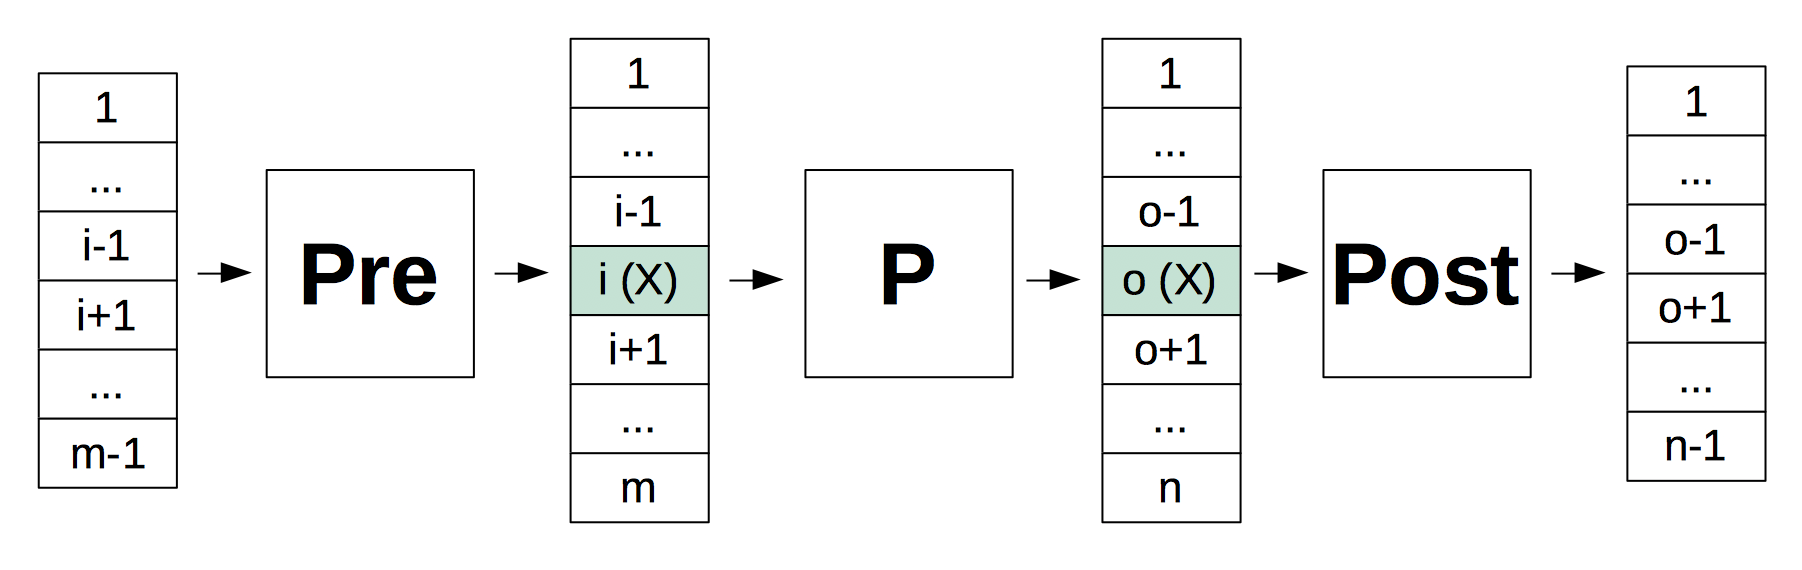
\includegraphics[scale=0.45]{feedback}
    \end{center}
    \caption{Feedback}
    \label{fig:feedback}
\end{figure}

\begin{theorem}[Monotonicity]
    Provided 
    \begin{align*}
        \begin{array}[]{ll}
        \healthy{SimBlock}\left(m_1, n_1, P_1\right) & \qquad \healthy{SimBlock}\left(m_1, n_1, P_2\right) \\
        P_1 \refinedby P_2 & \qquad i_1 < m_1 \land o_1 < n_1 \\
        \end{array}
    \end{align*}
    then,
    \begin{align*} 
       \left(P_1~f_D~(i_1, o_1)\right) \refinedby \left(P_2~f_D~(i_1, o_1)\right)
    \end{align*}
    \label{thm:fd_mono}
\end{theorem}
The monotonicity law states that if a block is a refinement of another block, then its feedback is also a refinement of the same feedback of another block. 

\begin{theorem}[Expansion]
    Provided 
    \begin{align*}
        \begin{array}[]{ll}
            P = FBlock\left( \logtrue{f}, m, n, f\right) & \qquad \healthy{SimBlock}\left(m, n, P\right) \\
            Solvable\_unique(i, o, m, n, f) & \qquad is\_Solution(i, o, m, n, f, sig) \\
        \end{array}
    \end{align*}
    then,
    \begin{align*} 
       & \left(P~f_D~(i, o)\right) & \\
       & = FBlock\left( \logtrue{f}, m-1, n-1, 
       \left(\lambda x, n @ \left(f\_PostFD(o) \circ f \circ f\_PostFD (sig, x, i)\right)~x~n\right)\right) & \tag*{[Expansion]}\\
      & \healthy{SimBlock}\left(m-1,n-1,\left(P~f_D~(i, o)\right)\right) & \tag*{[\healthy{SimBlock} Closure]}
    \end{align*}
    \label{thm:fd_exp}
\end{theorem}
In the expansion theorem, where 
\begin{definition}[$Solvable\_unique$] \label{def:solvable_unique}
    \begin{align*}
       & Solvable\_unique\left(i, o, m, n, f\right) \defs \\
       & \left(
       \begin{array}[]{l}
          \left(i < m \land o < n\right) \land  \\
            \left(\forall sigs @ \left(
                \begin{array}[]{l}
                    \left(\forall nn @ \#\left(sigs~nn\right) = (m - 1)\right) \implies \\
                    \left(\exists_1 sig@\left(\forall nn @ \left(sig~nn = \left(f \left(\lambda n1@ f\_PreFD\left(sig, i, sigs, n1\right), nn\right)\right)!o\right)\right)\right)
                \end{array} \right)\right)
       \end{array}
       \right)
    \end{align*}
\end{definition}
The $Solvable\_unique$ predicate characterises a condition that the block with feedback has a unique solution that satisfies the constraint of feedback: the corresponding output and input are equal. 

\begin{definition}[$is\_Solution$] \label{def:is_solution}
    \begin{align*}
       & is\_Solution\left(i, o, m, n, f,sig\right) \defs \\
       &\left(
       \begin{array}[]{l}
            \left(\forall sigs @ \left(
                \begin{array}[]{l}
                    \left(\forall nn @ \#\left(sigs~nn\right) = (m - 1)\right) \implies \\
                    \left(\forall nn @ \left(sig~nn = \left(f \left(\lambda n1@ f\_PreFD\left(sig, i, sigs, n1\right), nn\right)\right)!o\right)\right)
                \end{array} \right)\right)
       \end{array}
       \right)
    \end{align*}
\end{definition}
The $is\_Solution$ predicate evaluates a supplied signal to check if it is a solution for the feedback.

The expansion law of feedback assumes the function $f$, that is used to define the block $P$, is solvable in terms of $i$, $o$, $m$ and $n$. In addition, it must have one unique solution $sig$ that resolves the feedback. 

Our approach to model feedback in designs enables reasoning about systems with algebraic loops. If a block defined by $FBlock$ and $Solvable\_unique\left(i, o, m, n, f\right)$ is true, then the feedback composition of this block in terms of $i$ and $o$ is feasible no matter whether there are algebraic loops or not.

\subsection{Composition Examples}
For the compositions in Figure~\ref{fig:compose}, their corresponding maps in our design theory are shown below.
\begin{itemize}
    \item Figure~\ref{fig:id}: $\left(B_1 \parallel_B Id\right) \dcomp B_2$ 
    \item Figure~\ref{fig:split}: $Split2 \dcomp \left(B_1 \parallel_B B_2\right)$ 
    \item Figure~\ref{fig:router}: $\left(Split2 \parallel_B Split2\right) \dcomp Router(4, [0,2,1,3]) \dcomp \left(B_1 \parallel_B B_2\right)$ 
    \item Figure~\ref{fig:seq_comp}: $B_1 \dcomp B_2$ 
    \item Figure~\ref{fig:par_comp}: $B_1 \parallel_B B_2$ 
    \item Figure~\ref{fig:fd_comp}: $B~f_D~(0, 0)$ 
\end{itemize}
